

% Given
%  this definition, we have:
% %
% \begin{code}
%   map f . map g
% = {unfold map}
%   traverse id (f.) . traverse id (g.)
% = {eta expansion}
%   \arr -> traverse id (f.) . traverse id (g.) $ arr
% = {unfold traverse}
%   \arr -> traverse id (f.) (Delayed (id sh) (g.h))
%     where (sh, h) = delay arr
% = {unfold delay & traverse}
%   \arr -> (Delayed (id (id sh)) (f.g.h))
%     where (sh, h) = delay arr
% = {fold delay & traverse}
%   \arr -> traverse (id.id) ((f.g).) arr
% = {id.id = id & eta reduction}
%   traverse id ((f.g).) arr
% = {fold map}
%   map (f.g)
% \end{code}
% %
% Note that the use of delayed arrays combines successive array traversals into one, and that these traversals can have index space transformations before, in-between or after them. All this can be gained simply by inlining, as the definition of @map@ and other such traversals is non-recursive.
% 
% \subsection{Getting work done} % (fold)
% \label{sub:getting_work_done}
% 
% The fact that traversals can be delayed raises the question of when they will actually be triggered. This happens in one of two situations: (1) whenever we use an operation that combines or extracts elements from an array, such as reduction or indexing, and (2) when we explicitly use @force@.  In both situations, the traversals will be executed in parallel. This is discussed further in Section 7.
% We have already seen from the @mmMult@ example in Section~\ref{sub:combining_the_two}, that @force@ can be used to trigger the redistribution of array elements in order to facilitate cache-friendly array traversals. There is also a second situation where we want to @force@ the creation of manifest arrays.  


% \manuel{This is some older material from SPJ.  It is an interesting idea, but it is not what we are doing now and it is not what we have benchmarked.  So, I guess we should leave it out for now.}
% \manuel{Given we probably cannot take this route, we should probably have another subsection that talks about where to place @force@.  Right?}
% 
% \begin{verbatim}
% ============== PROBABLY HAS TO GO =================
% \end{verbatim}
% Where should these \texttt{force} operations be placed?  Our library puts them in
% by default, and omits them selectively when, as in the case of \texttt{transpose}
% we are confident that that duplicated work is cheaper than allocating an intermediate 
% array.  So the actual definition of \texttt{map} is more like this
% \begin{code}
% map f = force . traverse id (f.)
% \end{code}
% Does that mean the that map/map fusion we advertised above does not take place?
% No: it can still take place \emph{when the frozen array is consumed linearly}.
% This knowledge can be encapsulated in a rewrite rule:
% \begin{code}
%   RULE "map/force" forall f a.
%     map f (force a) = map f a
% \end{code}
% You might think that we need a rule for \texttt{map}, another for \texttt{scan} and so on,
% but it is easy to avoid this duplication.  Here is another definition of \texttt{map}
% \begin{code}
% map f arr = force (MkDArr (\i -> f (idx i)))
%           where
%             idx = unfreeze arr
% \end{code}
% where \texttt{unfreeze} has the obvious definition and rewrite rule
% \begin{code}
%   unfreeze :: DArray sh e -> sh -> e
%   unfreeze (MkDArr idx) = idx
% 
%   RULE "unfreeze/freeze" forall a.
%     unfreeze (freeze a) = unfreeze a
% \end{code}
% 
% \begin{verbatim}
% ========== End of PROBABLY HAS TO GO ==============
% \end{verbatim}

% subsection getting_work_done (end)


% 
% % -----------------------------------------        
% \section{Examples}
% 
% \manuel{All material from this section should be moved earlier and this section
% being disolved.}
% 
% 
% \subsection{Matrix-matrix multiplication}
% 
% \slpj{Do we really want to encourage our users to use traverse2DArray?
% Should we not jump straight to shorter, nicer code near the end.}
% 
% As a simple example, consider matrix-matrix multiplication. We can
% either implement it by directly manipulating the array function, or
% use the operations provided by the DArray library. Let as start with
% the former, which is more fairly similar to what we would write using
% loops over array indices:
% 
% \begin{code}
% mmMultP:: 
%   DArray (.,.)  Double -> DArray (.,.)  Double -> DArray (.,.)  Double  
% mmMultP arr1 arr2 =
%   fold (+) 0 arr'
%   where 
%     arr' = traverse2DArray arr1 arrT 
%       (\(sh*, m1, n1) -> \(_, n2, m2) -> (sh*, m1, n2, n1))
%       (\f1 -> \f2 -> \(sh*, i, j, k) -> f1 (sh*, i, k) * f2 (sh*, k, j))
% \end{code}
%      
%      In the first step, we create the intermediate three dimensional
%      array which contains the products of all sums and rows, and in
%      the second step, we collapse each of the rows to it's sum, to
%      obtain the two dimensional result matrix. It is important to note
%      that the elements of arrDP are never all in memory (otherwise,
%      the memory consumption would be cubic), but each value is
%      consumed immediately by mapfold.
% 
%      This implementation suffers from the same problem a corresponding
%      C implementation would - since we access one array row-major, the
%      other column major, the locality is poor. Therefore, first
%      transposing arr2 and adjusting the access will actually improve
%      the performance significantly:
% 
% \begin{code}
% mmMultP arr1 arr2 =
%   fold (+) 0 arr'
%   where 
%     arrT = forceDArray $ transpose arr2
%     arr' = traverse2DArray arr1 arrT 
%       (\(sh*, m1, n1) -> \(_, n2, m2) -> (sh*, m1, n2, n1))
%       (\f1 -> \f2 -> \(sh*, i, j, k) -> f1 (sh*, i, k) * f2 (sh*, j, k))
% 
% transpose:: DArray DIM2 Double -> DArray DIM2 Double  
% transpose arr = 
%   traverseDArray arr
%      (\(m,n) -> (n,m))
%      (\f -> \(i,j) -> f (j,i))
% \end{code}
% 
% 
% However, we do need to force the actual creation of the transposed
% array, otherwise, the change would have no effect at all. We therefore
% use forceDArray, which converts it into an array whose array function
% is a simple indexing operation (see description of forceDArray
% above). This means that the second version requires more memory, but
% this is offset by improving the locality for each of the
% multiplications.
% 
% As it is, mmMult can only take two-dimensional arrays as arguments,
% and is not mappable. If we look at the implementation closely, we can
% see that the restriction to two-dimensional arrays is unnecessary. All
% we have to do to generalise it is to adjust the type signatures and
% replace Z with an arbitrary shape variable:
% 
% \begin{code}
% mmMult1::
%   DArray (d*,.,.)  Double-> 
%     DArray (d*,.,.)  Double-> 
%     DArray (d*,.,.)  Double  
% mmMult1 arr1 arr2 = 
%   fold (+) 0 arrDP
%   where 
%     arr2T = forceDArray \$ transpose arr2
%     arrDP = traverse2DArray arr1 arrT 
%       (\(sh*, m1, n1) -> \(_, n2, m2) -> (sh*, m1, n2, n1))
%       (\f1 -> \f2 -> \(sh*, i, j, k) -> f1 (sh*, i, k) * f2 (sh*, j, k))
% 
% transpose:: DArray (d*,.,.) a -> DArray (d*,.,.)  a
% transpose arr =
%   traverseDArray arr
%      (\(sh*,m,n) -> (sh*,n,m))
%      (\f -> \(sh*,i,j) -> f (sh*,j,i))
% \end{code}
% 
% An alternative way to define matrix-matrix multiplication is in terms
% of the collective library functions provided. First, we expand both
% arrays and, in case of arr2 transpose it such that the elements which
% have to be multiplied match up. Then, we calculate the products using
% zipWith, and then use fold to compute the sums:
% 
% \begin{code}
% mmMult2:: 
%     DArray (d*,.,.)  Double-> 
%     DArray (d*,.,.)  Double-> 
%     DArray (d*,.,.)  Double  
% mmMult2 arr1 arr2 =
%   fold (+) 0 (arr1Ext * arr2Ext)
%   where
%     arr2T   = forceDArray \$ transpose arr2  
%     arr1Ext = replicate arr1 (*,m2,*)
%     arr2Ext = replicate arr2T (*,*,n1)              
% \end{code}
% \slpj{what are n1, n2?}
%              
% In this implementation, transpose is necessary to place
% the elements at the right position for zipWith, and we
% call forceDArray for the same reason as in the previous
% implementation, to improve locality. Also, mmMult2'
% outperforms mmMult1, as the use of replicate` exposes
% the structure of the communication, whereas the general
% index calculations in mmMult1 hide this structure, and
% thus are less efficient.



% \subsection{Red-Black Gaussian Relaxation}
% \begin{code}
% redBlack:: Double-> Double-> DArray (d*,.,.,.) Double->
%   DArray (d*,.,.,.) Double -> DArray (d*,.,.,.) Double
% redBlack factor hsq f arr  = 
%   applyFactor $ insert odd arr' $ sumD $ 
%     getBlack $ stencil arr'

%   where
%     (d*, l, n, m) = darrayShape arr
%     arr' =  
%       applyFactor $ insert even arr $ sumD $ 
%       getRed $ stencil arr

%     applyFactor = 
%       zipWith (\fi -> \si -> factor *  (hsq * fi + si)) f
    
%     sumD arr = fold (+) 0 arr 
 
%     getRed arr = traverseDArray arr
%        (\(sh*, l, m, n, c) -> (sh*, l-2, m-2, (n-1)`div` 2, c))
%        (\f -> \(sh*, h, i, j, c) -> f(sh*, h+1, i+1, 2*j+1, c)) 

%     getBlack arr = traverseDArray arr
%         (\(sh*, l, m, n, c) -> (sh*, l-2, m-2,  (n-2) `div` 2, c))
%         (\f -> \(sh*, h, i, j, c) -> f (sh*, h+1, i+1, 2*j+2, c)) 

%     isBorder (_, h, i, j) = ((h * i * j) == 0)  || 
%       (h >= (l-1)) || (i >= (m-1)) || (j >= (n-1))

%     insert p arr1 arr2 (DArray sh f) (DArray sh' f')  =
%       traverse2DArray arr1 arr2 (\d -> \_ -> d)
%          (\f1 -> \f2 -> \(sh*, h, i, j) -> 
%             if ((isBorder (sh*, h, i, j)) || p j) 
%               then f1 d 
%               else (f2 (sh*, h-1, i-1, (j-1)`div` 2)))

%     stencil arr = traverseDArray (\(sh*,k,l,m) -> (sh*,k,l,m,6))
%       (\f -> f' 
%          where 
%            f' (sh*, n, m ,0) = f (sh*, n, m+1)
%            f' (sh*, n, m, 1) = f (sh*, n, m-1)
%            f' (sh*, n, m, 2) = f (sh*, n+1, m)
%            f' (sh*, n, m, 3) = f (sh*, n-1, m)
%            f' (sh*, k, n, m, 4) = f (sh*, k+1, n, m)
%            f' (sh*, k, n, m, 5) = f (sh*, k-1, n, m))

%       \end{code}
 

% Compared to the C version of the Laplace solver, our sequential
% version is 22\% slower, and the parallel version run on a single
% thread is 53\% slower.  
% The parallel Laplace solver on the Xeon achieves an absolute speed up
% of 1.7, and a relative speed up of about 2 on the Xeon's eight
% processors. The poor scalability on this architecture is
% due to its limited bandwidth and the memory bound nature of
% this algorithm. In contrast, on the T2 the same program achieves a
% relative speed up of almost seven on eight processors.
%
% The following table contains the running times in milliseconds of
% mmMult1 and mmMult2', applied to two matrices of with size * size
% elements. As mentioned before, mmMult2 is faster than mmMult1, as
% replicate can be implemented more efficiently than the general
% permutation which is the result of the element-wise index computation
% in mmMult1. This is the case for most problems: if it is possible to
% use collection oriented operations, than it will lead to more
% efficient code. We can also see that using forceDArray for improved
% locality has a big impact on performance (we have O (size*size*size)
% memory accesses, and creating the transposed matrix has only a memory
% overhead of O(size*size)). mmMult1` without the transposed matrix is
% about as fast as mmMult2 without forceDArray (times omitted). We can
% also see that the speedup on two processors is close to the optimal
% speedup of 2.
%
% To get an idea about the absolute performance of DArrays, we compared
% it to two C implementations. The first (handwritten) is a straight
% forward C implementation with three nested loops, iterations
% re-arranged to get better performance, which has a similar effect on
% the performance than the forceDArray/transpose step. The second
% implementation uses the matrix-matrix multiplication operation
% provided by MacOS accelerate library. We can see that, for reasonably
% large arrays, DArrays is about a factor of 3 slower than the C
% implementation if run sequentially.
% \begin{figure}
% 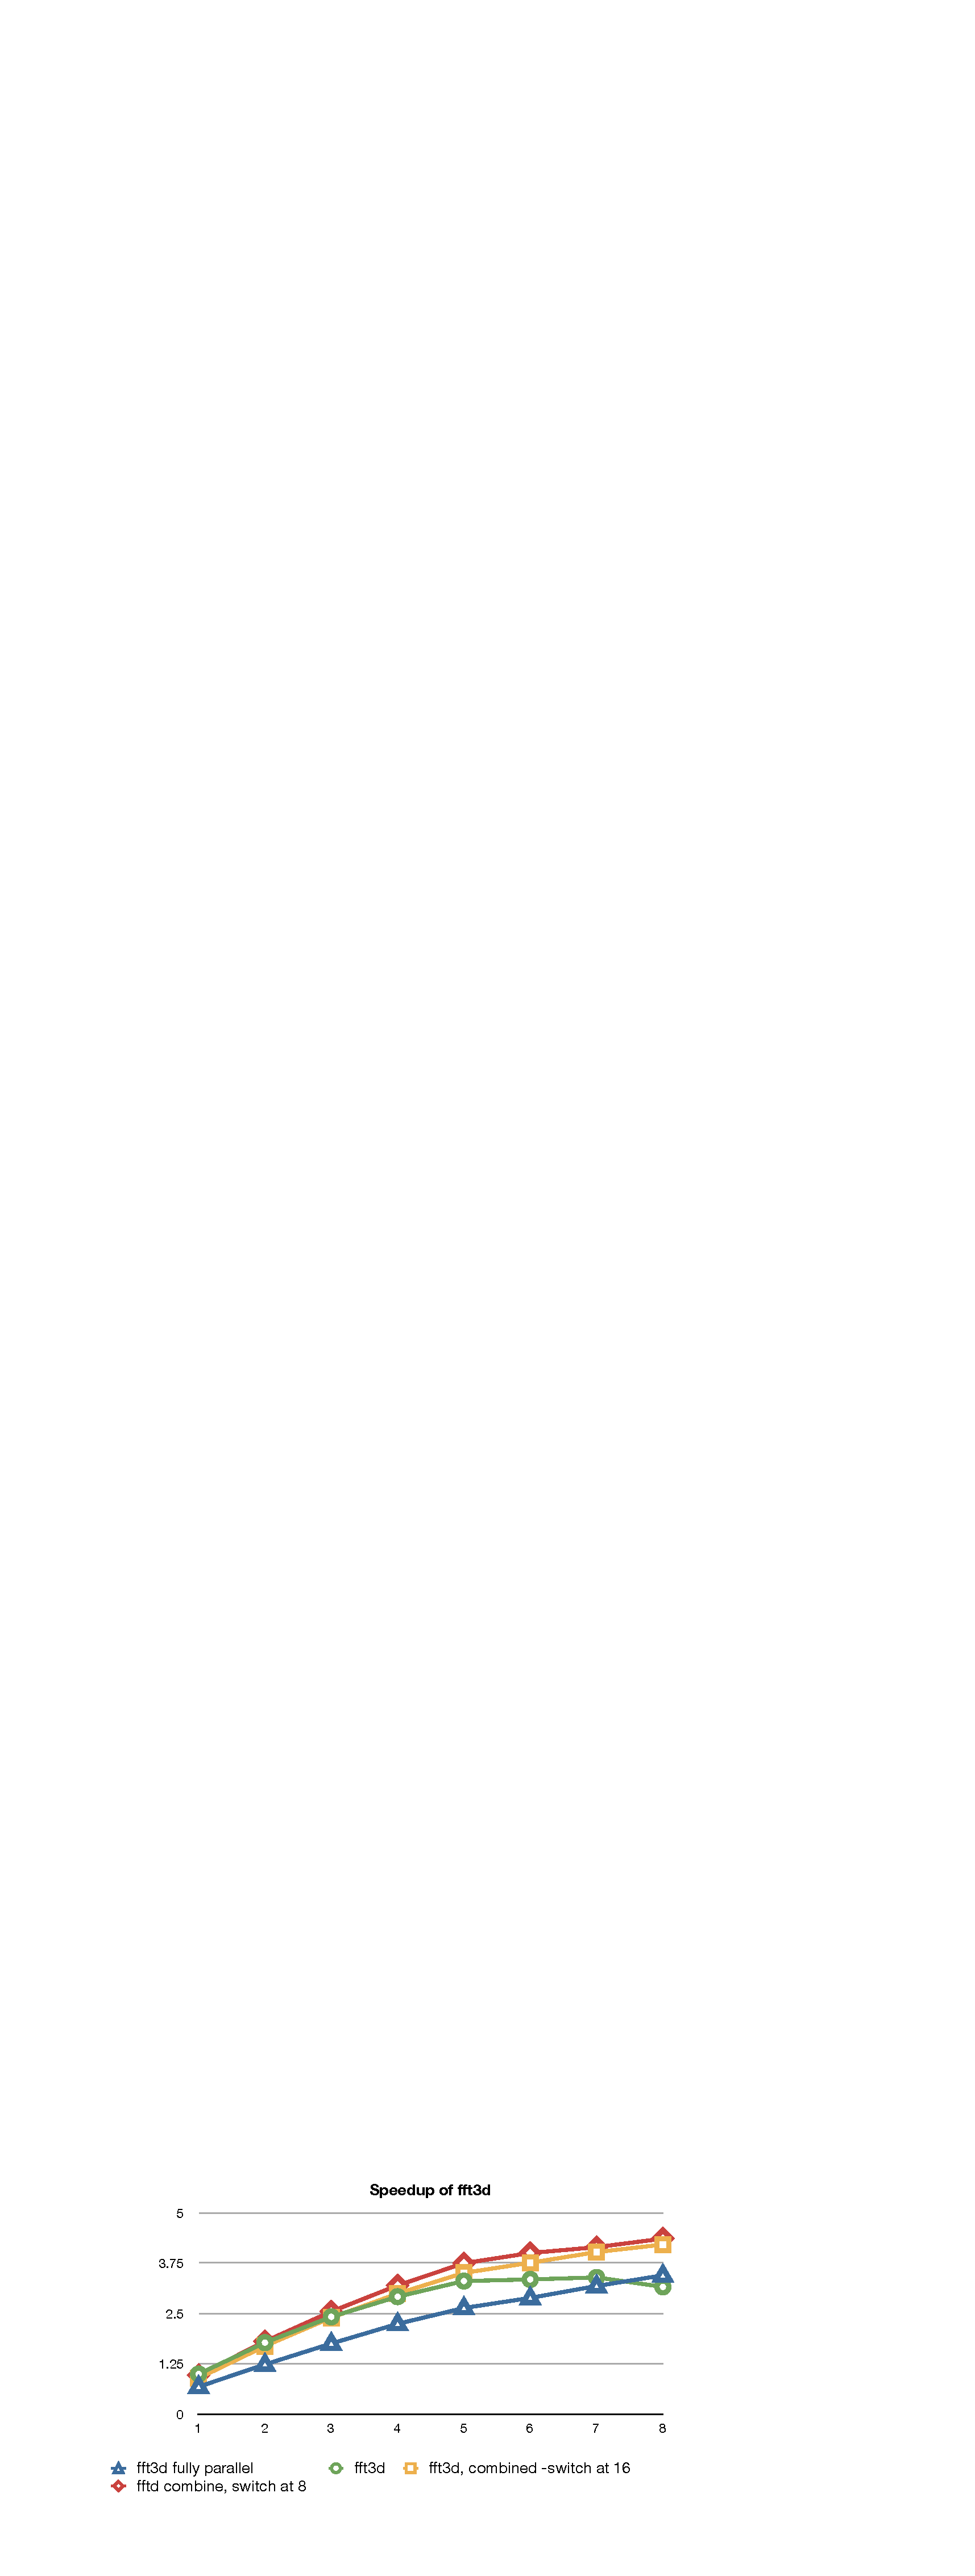
\includegraphics[width=0.5\textwidth]{./Benchmarks_fftSpeedupCmp.pdf}
% \caption{3-dimensional FFT}
% \label{MMult}
% \end{figure}






% \begin{small}
% \begin{code}
%   ----------------------------------------------------------------------
%   size                            |       256 |       512 |    1024 | 
%   ----------------------------------------------------------------------    
%   mmMult1                         |       675 |      5323 |   42674 |
%   ----------------------------------------------------------------------
%   mmMult2                         |       345 |      2683 |   21442 |
%   ----------------------------------------------------------------------
%   mmMult2  (2PE)                  |       190 |      1463 |   11992 |
%   ----------------------------------------------------------------------
%   mmMult2 (w/o forceDArray)       |       974 |      8376 |   73368 |
%   ----------------------------------------------------------------------
%   mmMult2 (w/o forceDArray, 2PE)  |       508 |      4368 |   37677 |
%   ----------------------------------------------------------------------
%   C (hand written)                |        34 |       514 |    7143 |
%   ----------------------------------------------------------------------
%   C (MacOS Accelerated Vector)    |        33 |       510 |    6949 |
%   ----------------------------------------------------------------------

% mmMult2 auf Limiting factor, 1024*1024 elemente

% PEs   milliseconds
% 1     23271
% 2     11954
% 3     8242
% 4     6354
% 5     5184
% 6     4395
% 7     3905 
% 8     3503



% fft3d 64

% 1 2005
% 2 1107
% 3 780
% 4 610
% 5 519
% 6 474
% 7 430
% 8 397


% fft3d 32

% 1 187
% 2 100
% 3 76
% 4 62
% 5 53
% 6  52
% 7 51
% 8 51
  



% fft3ds 64

% 1 1370
% 2 779
% 3 566
% 4 469
% 5 414
% 6 409
% 7 403
% 8 433


% fft3ds 32

% 1 140
% 2 93
% 3 73
% 4 65
% 5 60
% 6 58
% 7 65
% 8 72 


% fft3dC 64, switch at 16


% 1 1529
% 2 809
% 3 571
% 4 457
% 5 390
% 6 364
% 7 342
% 8 325 


% fft3dC 64, switch at 8
% 1 1402
% 2 757
% 3 537
% 4 428
% 5 365
% 6 342
% 7 339
% 8 314 


% \end{code}
% \end{small}
% \subsection{Red-Black Gaussian Relaxation}


% \subsection{Notation}

% \slpj{I'm very dubious about this notation.  I don't think it buys us
% much, and it's verbose (and still imprecise) to explain.  I suggest
% doing without it.}

% {\em % --------------------------------------
% Defining the shape type inductively has the advantage that we can do
% some computations on the type level, and we can easily express
% conditions like 'at least of rank 1'. It is, however, quite
% inconvenient for the user having to write \texttt{(Z :*: 3 :*: 4)}
% instead of just \texttt{(3,4)} or \texttt{[3,4]} to describe a
% concrete shape. So, we want to use the nested representation
% internally, but hide it from the user. For this, we could either use
% type families to distinguish between the external (convenient) and the
% internal (but awkward) representation type, or by adding syntatic
% sugar. As the de-sugarer is already used to handle other DPH specific
% notation, this is not much of an additional overhead.  We haven't
% implemented either yet, but for sake of a clearer presentation in this
% paper, we use the following notation:

% \begin{itemize}

% \item a shape type of rank n is represented by an n-tuple of dots separated
%   by commata, e.g., \texttt{(.)} instead of \texttt{Z :*: Int} for a
%   one-dimensional array, \texttt{(.,.)} for a two dimension array, and
%   so on.

% \item a shape type of at least rank n is represented by an $n+1$ tuple, where
%   the first element is a regular type variable identifier, followed by
%   an asteriks, followed by $n$ dots.  For example, if the first argument of
% a function is an array with at least rank 1, we can either write
% \begin{code}
%   f:: Shape d => DArray (d :*: Int) .....
% \end{code}
%   or, more concisely
% \begin{code}
%   f:: DArray (d*, .) .....
% \end{code}

% There can only be at most one shape type variable, always at the
% leftmost position in the tuple.
% \end{itemize}

% With this, the type of the functions discussed above change to:
% \begin{code}
%   toScalar:: Elt e => 
%     DArray Z e -> e
%   map:: (Elt a, Elt b)  => 
%     (a -> b) -> DArray (d*) a  -> DArray (d*) b
%   sum:: Num a => 
%     DArray (d*,.) a  -> DArray (d*) a
% \end{code}

% Similarly on the value level for shapes and indices into an array:
% \begin{itemize}

% \item a shape of rank n is represented by an n-tuple of expressions,
%   separated by commata, e.g., \texttt{(5)} instead of \texttt{Z :*:
%     5} for a one-dimensional array of length $5$ (or an index to the
%   6th element of a one dimensional array), \texttt{(2, 3)} to denote
%   the shape of a two by three matrix, and so on.

% \item a pattern for a shape of at least rank n is represented by an
%   n+1 tuple, where the first element is a regular variable identifier,
%   followed by an asteriks, followed by a comma  separated
%   list of expressions.  For example, if we match on the shape of the argument of
% \texttt{f} in the example above, instead of writing
% \begin{code}
%   f:: Shape d => DArray (d :*: Int) .....
%   f arr .. = 
%      where (sh :*: n) = darrayShape arr

% \end{code}
%   we now write
% \begin{code}
%   f:: DArray (d*, .) .....
%   f arr .. = 
%      where (sh*, n) = darrayShape arr
% \end{code}
% There can only be at most one shape variable in a shape, always at the
% leftmost position in the tuple.
% \end{itemize}

% } % ------------------ end of \em --------------------
